%!TEX root = ../thesis.tex

\chapter{Proposed Architecture} % Main chapter title

\label{chapter:Architecture} % Change X to a consecutive number; for referencing this chapter elsewhere, use \ref{ChapterX}

\lhead{Chapter 9 \emph{Proposed Architecture}} % Change X to a consecutive number; this is for the header on each page - perhaps a shortened title

%----------------------------------------------------------------------------------------
%	SECTION 1
%----------------------------------------------------------------------------------------

\section{Technology Choices}

\subsection{Java Language}
Java is a general-purpose computer programming language that is concurrent, class-based, object-oriented, and specifically designed to have as few implementation dependencies as possible. It is also a cross-platform language which means that it would be possible to use it without any recompilation needed. Java is very easy to use, well documented a has the support of a large community (more than 9 million developers reported). Therefore, lot of libraries are available, we will present some of them below. 

\subsection{Neo4j}
Graph-based databases are very intuitive to work with and allow the user to model the world as he experience it. The model schema isn't rigid and the user can edit it at anytime, adding new entities or new kind of relationships. Neo4j is an open-source graph database, implemented in Java (so cross-platform), maturing for 15 years and currently running version 2.2. It is the most popular graph database nowadays\footnote{http://db-engines.com/en/ranking/graph+dbms}, has a great scalability, a strong community and has its own query language : Cypher. 

\subsection{DBpedia Spotlight} % (fold)
\label{sub:dbpedia_spotlight}
As presented in \ref{sub:dbpedia}, DBpedia propose a nice tool to automatically annotating mentions of DBpedia resources in text : DBpedia Spotlight. We chose to use it even if we can't exploit its full potential since we don't have a context. Its usage is really simple and performances are quite ok given our use-case. See Code \ref{code:spotlight} for a sample response.
% subsection dbpedia_spotlight (end)

\subsection{Semantic Resources Libraries} % (fold)
\label{sub:semantic_resources_libraries}
We needed to access the chosen online ontologies (DBpedia's and WordNet's) from our prototype. To achieve this, we used the fact that Java is very popular and lot of libraries are available.
\paragraph{JENA} % (fold)
\label{par:jena}
We chose Apache JENA ARQ\footnote{https://jena.apache.org/documentation/query/index.html} to query the RDF-base schema of DBpedia. This solution is stable and maintained by a famous structure : Apache. Using it was really simple.
% paragraph jena (end)
\paragraph{JAWS} % (fold)
\label{par:jaws}
Regarding WordNet, we used JAWS\footnote{http://lyle.smu.edu/~tspell/jaws/} which has been developed and is maintain by a member of the Southern Methodist University (Dallas, Texas). Its last version is a bit old but this isn't an issue since WordNet's upgrades have also stopped. This library was also deeply intuitive and easy to use.
% paragraph jaws (end)
% subsection semantic_resources_libraries (end)
\subsection{JSoup} % (fold)
\label{sub:jsoup}
Our two last experiments are based on Wikipedia's web-pages. Therefore we needed a way to crawl and extract content from them. The JSoup\footnote{http://jsoup.org/} library was a perfect asset to achieve this. It is open-source, implements the WHATWG HTML5 specification, and parses HTML to the same DOM as modern browsers do. It also allows the user to build specific queries to access particular elements in the DOM.
% subsection jsoup (end)

\subsection{Stanford NLP} % (fold)
\label{sub:stanford_nlp}
Crawling web-pages is a thing, but extracting relevant data from it is another one. The Stanford NLP Research Group\footnote{http://nlp.stanford.edu/} has released several libraries in different programming languages including Java. Those libraries can achieve many things such as sentence segmentation, Part-of-speech (POS) tagging, named entities recognition and so on\dots We used the POS Tagger to extract nouns from Wikipedia paragraphs.
% subsection stanford_nlp (end)

\section{Graph Structure} % (fold)
\label{sec:graph_structure}

\subsection{Vertexes} % (fold)
\label{sub:vertexes}
Each vertex represents a semantic concept (virtual or real).\\
Virtual ones are concepts created in purpose to perform operations. Here we’re talking about 2 different kinds of nodes :
\begin{itemize}
	\item Base concepts : those are created in order to represent the originals tags. Their URIs follow this pattern : “base:TAG” (ex : base:dog) and their \emph{TAG} value is lemmatized (dogs -$>$ dog).
	\item Top/Bottom concepts : these two concepts (virtual:top and virtual:bottom) are essential in the compuation of the Wu-Palmer evolved measure (see \ref{ssub:evolved_wu_palmer}).
\end{itemize}
Real nodes are semantic nodes linked to entities, classes (DBpedia) or synsets (WordNet):
\begin{itemize}
	\item WordNet's nodes pattern : “Wordnet:TAG” (ex: Wordnet:plant)
	\item DBpedia's nodes pattern : “DPedia’s concept URI”\\(ex: http://dbpedia.org/resource/London)
\end{itemize}
% subsection vertexes (end)

\subsection{Edges} % (fold)
\label{sub:edges}
There are 3 kind of edges :
\begin{itemize}
	\item VIRTUAL : represent virtual links between nodes, not present in any of the semantic resources, created by the algorithm
	\item EQUIV : represent an equivalence between nodes from 2 different ontologies \\
	(ex : http://dbpedia.org/resource/Dog and Wordnet:dog)
	\item PARENT : represent a semantic link which is of type “IS-A” (implemented by the rdfs:subClassOf predicate in DBpedia and the hyperonym/holonym relation in WordNet)
\end{itemize}
% subsection edges (end)

\subsection{Construction} % (fold)
\label{sub:construction}
Now that we have described our graph, we will present how it is built.\\

Given an initial set of input tags, the first step of our construction process is to detect semantic concepts among them. To achieve this, we use DBpedia Spotlight (shortly presented in \ref{sub:dbpedia_spotlight}) and its REST endpoint. It takes as input a string (here the list of tags, separated by commas) and returns a JSON object containing detected semantic concepts, see Code \ref{code:spotlight} for a sample response. We then use the JAWS library and request all input tags to our WordNet database. This returns us a list of synsets.\\

\lstinputlisting[language=json,caption=DBpedia Spotlight sample response,float,label={code:spotlight}]{./Primitives/sampleDBpediaSpotlight.json}
We have now to create the hierarchical tree for each of this base concepts and stop when we reach the ontology's root. In order to do so, we again split the task according to the ontology the concept comes from. For DBpedia's, we send SPARQL requests through the JENA library. Code \ref{code:entity} if the resource is an entity and we need to find its class. Code \ref{code:class} if the resource is a class and we so need to find it's superclass.\\
\lstinputlisting[language=SPARQL,caption=Find entity's class,float,label={code:entity}]{./Primitives/entity.sparql}
\lstinputlisting[language=SPARQL,caption=Find class' superclass,float,label={code:class}]{./Primitives/class.sparql}
It is a bit more simple with the WordNet's concepts. Since we have the initial synsets, we can easily navigate into them and extract hypernyms. This whole process is recursive, for each new concept we start again.\\

The last step of our process is the detection of equivalences. To do so we start from the DBpedia's nodes, get their label and request WordNet. If a correspondence is found, then we create the equivalent node, interlink it via an EQUIV edge to the initial one and build its generalization tree as presented above.\\

An extract of our constructed graph is presented in figure \ref{fig:graph}. It comes from the browser interface of Neo4j and we can here see all kind of nodes and relationships. More precisely, the bottom-left node is \emph{virtual:bot} and the top-right is \emph{virtual:top}. Between them, we chose to display two initial tags (\emph{base:chapel} and \emph{base:cologne cathedral}) and their generalizations. We can observe an \emph{EQUIV} relation between the red (\emph{http://dbpedia.org/ontology/Building}) and the green (\emph{Wordnet:building}) circles. Both WordNet and DBpedia ontologies' root are displayed in the blue circles (\emph{Wordnet:entity} and \emph{http://www.w3.org/2002/07/owl\#Thing}) and linked to our \emph{virtual:top} root.
% subsection construction (end)

\begin{figure}[h]
\begin{center}
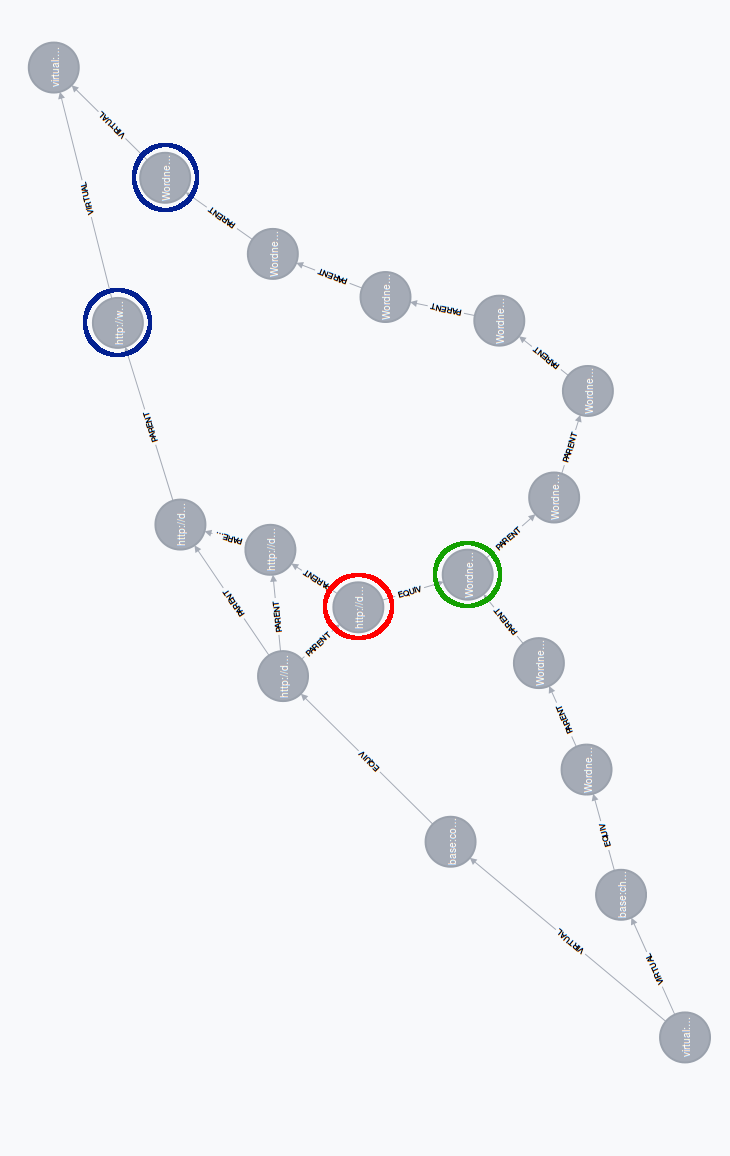
\includegraphics[scale=0.55]{./Primitives/graphExtract.png}
\end{center}
\caption{Graph extract}
\label{fig:graph}
\end{figure}

\subsection{Pro-Cons} % (fold)
\label{sub:pro_cons}
This graph-based model approach has several benefits : it is more intuitive to imagine the inheritance of a concept, the computation of basic metrics such as shortest path between two concepts or their Least Common Subsumer (LCS) is really easy, the schema isn't rigid and has, in fact, evolved during the project \dots\\

However, our choice also has drawbacks : No disambiguation system has been implemented which means that all parents of a node are added to the graph making it always bigger and slower to browse. Given the graph's size and my machine performances, the integration of the Wu-Palmer evolved measure wasn't possible (but implemented and tested on smaller graphs).
% subsection pro_cons (end)
% section graph_structure (end)

\section{Code and Procedure Explanations} % (fold)
\label{sec:code_and_procedure_explanations}
This work has been split into several Java projects, each completing a special task. In this section we will present these projects and detail their main classes.
\subsection{TreeGenerator} % (fold)
\label{sub:treegenerator}
This project achieve the creation of a data model representing our hierarchical concepts organization. We chose to create a Java object-based data model in order to be able to do different things with it, like importing it in a graph database.\\
It is split into one main class and two packages : 
\begin{itemize}
	\item \textbf{treegenerator.model} : This package contains all the classes that represent the entities of our project. These classes are organized as an inheritance schema where :
	\begin{itemize}
		\item \textbf{OnlineConcept} is the mother class which define the common attributes and initialize the \emph{parents} and \emph{childs} vectors. These vectors store all the concepts that are linked to this entity, as generalizations or specializations.
		\item \textbf{DBpediaConcept} inherit from OnlineConcept and define specific constructors which can either take a JSON object or an URI as input.
		\item \textbf{WordNetConcept} inherit from OnlineConcept, defines a specific constructor and stores the Concept associated synset.
		\item \textbf{TypeTerm} enumerate all the concept's types.
	\end{itemize}
	Each Concept can have multiple parents and multiple childs. Class diagram is available in Figure \ref{fig:tg_model}.
	\item \textbf{treegenerator.services} : This package contains three tools that we use for the data-model creation: 
	\begin{itemize}
		\item \textbf{SpotlightConnection} : This class operates the connection to DBpedia Spotlight's REST service, sending the initial tags as an input text and returning a JSON object.
		\item \textbf{WordNetConnection} : This class query our download WordNet version by retrieving the synsets associated to an input keyword.
		\item \textbf{Inflector} : This class performs the lemmatization process we presented in \ref{sec:global_process}. It is based on a list of regular expressions and extends an initial work from \emph{chuyeow}\footnote{https://github.com/chuyeow}.
	\end{itemize}
	\item \textbf{TreeGenerator} : The main class, which contains methods to generate the data-model. Few are important and are presented below :
	\begin{itemize}
		\item \textbf{run} : the main method, initialize all the parameters and start the construction process.
		\item \textbf{runAndGenerateGEXF} : same as above but also generate a GEXF\footnote{http://gexf.net/format/} file containing our data model.
		\item \textbf{getAncestors} : define all of our process' steps presented in \ref{sec:global_process}
		\item \textbf{recursionTerms} : the recursive function which is called for every new concept in order to build its generalization.
	\end{itemize}
\end{itemize}

\begin{figure}[h]
\begin{center}
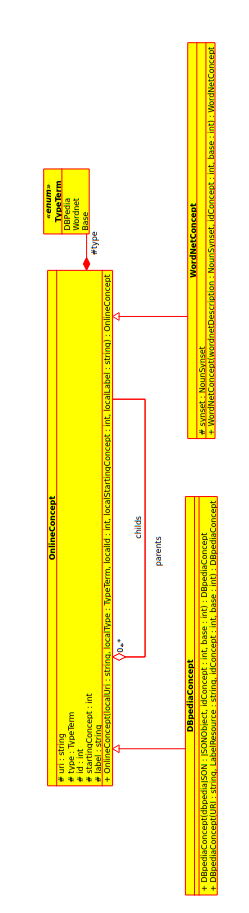
\includegraphics[scale=0.6]{./Primitives/treeGeneratorModel.png}
\end{center}
\caption{TreeGenerator class diagram}
\label{fig:tg_model}
\end{figure}
% subsection treegenerator (end)
\subsection{GexfParserForNeo4jDB} % (fold)
\label{sub:gexfparserforneo4jdb}
We won't detail this project since it has only be an interim project. Its aim is to parse a GEXF file and create a model in a Neo4j database. It is split into two packages :
\begin{itemize}
	\item \textbf{gexfparserforneo4jdb.gexf} : Parse the GEXF file into a Java Graph object.
	\item \textbf{gexfparserforneo4jdb.neo4j} : Connects to the Neo4j database and transform the Java Graph object in a Neo4j graph model. 
\end{itemize}
% subsection gexfparserforneo4jdb (end)
\subsection{SemObsNeo4j} % (fold)
\label{sub:semobsneo4j}
This project achieve several tasks. First it allows the user to connect to an external source of data (CSV file or PostgreSQL database) and run the generalization tree step by calling the TreeGenerator project (\ref{sub:treegenerator}).\\
Then it make use of the Java data-model created by TreeGenerator and directly parse it into a Neo4j graph without using an interim GEXF file. This whole creation phase can be repeated as much as the user wants, the nodes won't be created twice since we check for the existing ones before any upload operation.\\
Eventually, the project also run our experiments and compute the results into several files.\\
It is split into two packages each containing a lot of classes we will now present :
\begin{itemize}
  	\item \textbf{semopsneo4j} : This package contains the main class of our project and several useful hand-made tools.
  	\begin{itemize}
  		\item \textbf{SemObsNeo4j} : This class loads the properties of our project, initializes the Neo4j database if needed and starts the chosen task.
  		\item \textbf{SemDistance} : This class performs the calculation of semantic measures and propose several ways to export its results as matrices.
  		\item \textbf{DataReader} : This class connects to the external source of data and parse it into a Java Map object in which a key (the image's ID) is associated with an ArrayList of its tags.
  		\item \textbf{ModelImporter} : This class uses the data model created by TreeGenerator in order to build our graph model. It also checks for already existing concepts to avoid duplication.
  		\item \textbf{BFSTraverser} : This class implements a Breadth-First Search (BFS) algorithm using our graph structure. It is used in our graph-based experiments presented in \ref{sub:graph_based_experiments}.
  		\item \textbf{WikipediaCrawler} : This class crawl the content of a Wikipedia's page based on an input tag. Obviously, nothing is done if the requested URL doesn't exist.
  		\item \textbf{NLPParser} : This class performs several operations provided by the Standford NLP library already presented in \ref{sub:stanford_nlp}. We mainly use the Part-Of-Speech module which associate a label to each word. 
  		\item \textbf{PairNodeScore} : This class is a hand-made pair structure which contains a Node object and a double field. This allows us to store the detected candidates in our experiments and perform operations on them. 
  	\end{itemize}
  	\item \textbf{experiment} : This package contains our experiments classes and a main class for the whole evaluation step. We won't detail the experiments algorithms since it will be done in the next chapter. The experiments classes are organized as follows :
  	\begin{itemize}
  		\item \textbf{RelevantTagsExperiment} : The mother abstract class, define all common attributes such as the list of considered initial tags, the execution time or the selected candidates.\\
  		This class also contains the export methods, more about the exports will be presented in the next chapter.
  		\item \textbf{RelevantTagsExperimentDN} : Inherits from RelevantTagsExperiment and implements a direct parents search.
  		\item \textbf{RelevantTagsExperimentLists} : Inherits from RelevantTagsExperiment and implements a search based on lists of initial tags.
  		\item \textbf{RelevantTagsExperimentWL} : Inherits from RelevantTagsExperimentLists and implements a candidate's global score computation based on the whole list of initial tags.
  		\item \textbf{RelevantTagsExperimentSL} : Inherits from RelevantTagsExperimentLists and implements a candidate's global score computation based on sub-lists of initial tags.
  		\item \textbf{RelevantTagsExperimentWikiLinks} : Inherits from RelevantTagsExperiment and implements search among internal Wikipedia's links.
  		\item \textbf{RelevantTagsExperimentWikiContent} : Inherits from RelevantTagsExperiment and implements a search among all nouns in a Wikipedia's page first paragraph.
  	\end{itemize}
  	Class diagram of our experiments classes is available on Figure \ref{fig:exp_model}.
  \end{itemize}  

\begin{figure}[h]
\begin{center}
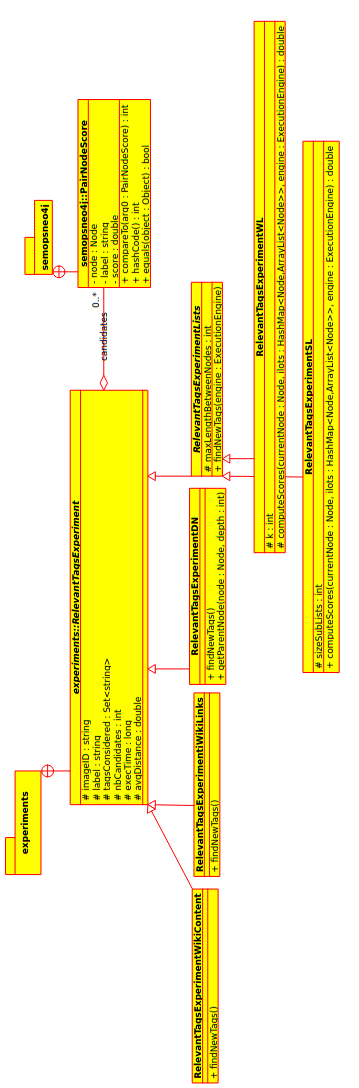
\includegraphics[scale=0.6]{./Primitives/experimentsModel.png}
\end{center}
\caption{Experiments class diagram}
\label{fig:exp_model}
\end{figure}
% subsection semobsneo4j (end)
% section code_and_procedure_explanations (end)